%File: formatting-instruction.tex
\documentclass[letterpaper]{article}
\usepackage{aaai}
\usepackage{times}
\usepackage{helvet}
\usepackage{courier}
\usepackage{hyperref}
\usepackage{comment}
\usepackage{graphicx}
\usepackage{natbib}
\usepackage{framed}

\usepackage{url}
\usepackage{hyperref}

\usepackage{amsmath,amsfonts,amsthm} % Math packages
\usepackage{algorithm}
%\usepackage{algorithmicx}
\usepackage[noend]{algpseudocode}
\usepackage{subfigure}

\frenchspacing
\setlength{\pdfpagewidth}{8.5in}
\setlength{\pdfpageheight}{11in}
\pdfinfo{
/Title (Community analysis on the social networks using Latent Dirichlet Allocation)
/Author (Daqing Yi)}
\setcounter{secnumdepth}{0}  
\begin{document}
% The file aaai.sty is the style file for AAAI Press 
% proceedings, working notes, and technical reports.
%
\title{Community analysis on the social networks using Latent Dirichlet Allocation}
%\subtitle{CS 660 Computer Networks}

\author{ 
	Joseph Walker 
	\\ \texttt{joseph.k.walker@gmail.com}
	\And Seung-Hee Yang 
	\\ \texttt{yangseung0105@gmail.com}
	\And Daqing Yi 
	\\ \texttt{dqyi11@gmail.com}
}
\maketitle

\begin{abstract}
Connecting the academic papers or the academic authors creates social network structures.
By different ways of connecting nodes, the social network structure can represent different relationship in academic society.
Using Latent Dirichlet Allocation to model the generative model of the network supports the analysis on the social network,
particular the network at large scale.
Our project collects academic documents from Google Scholar and creates corresponding social network structures.
After the generative model has been learned from social network structure,
many potential features could be extracted.
\begin{comment}
Many authors in academic circle publish their papers and their papers are published on-line.
Authors of the papers tend to form a network similar to online social networks.
Sites that hosts papers such as Google Scholar are popular, and their popularity provides an opportunity to study the characteristics of the document network at large scale.
Understanding the document network is meaningful in both improving the current document systems and designing new applications for the document network.
Our project presents a measurement study and analysis of the structure of document network by Google Scholar. 
\end{comment}
\end{abstract}

\section{Introduction}

Social networks, as an abstract of the relationship connections between a large scale of objects, exist in many groups of objects.
These groups of objects can persons, identities, documents, pictures and many more.
By figuring out the patterns and the features of a social network, people hope to explore the potential phenomenons in this society.
However, the huge amount of data makes the pattern analysis on this network structure a hard problem.
Recently, Latent Dirichlet Allocation~\cite{Blei:2003:LDA:944919.944937} , a popular technique applied in text mining, has been imported to the community analysis on the social networks.
In the text mining, LDA uses a Bayesian network structure for a document generative model.
The words in the documents are used as samples to training the Bayesian network.
The trained Bayesian network is expected to approximate the latent text data distribution, which could be used for pattern analysis purpose.
By modeling the social network distribution in a similar way, the Latent Dirichlet Allocation can be applied to analyze the social network structures
~\cite{4258697} \cite{Cha:2012:SAU:2348283.2348360} \cite{Henderson:2009:ALD:1529282.1529607}.

In this project, we explore the social networks inside the academic scholar database.
Among various types of information sharing systems provided in the Internet, online academic document database, such as Google Scholar and Microsoft Academic Search, have gained growing popularity.
As of 2014, Google Scholar is reported to contain around 160 million documents with Microsoft Academic Search containing around 40 million documents. 

The document networks are proposed to analyze the latent relationship between papers~\cite{chang2009relational}.
It connects the papers as a social network, in which the connection can be defined by citation, author, keyword, category and etc.
Also the academic scholar database also indicates a social network of the authors.
The authors are connected as a network by the papers, which can be determined by coauthor relationship, citation, academic institutions, academic conferences and etc.
Participating authors join the network, publish their brief profile.

An understanding for these types of social networks can help to read the important states of the current society.
For example, understanding the structure of the document networks may lead to algorithms that can detect influential authors.
In this project paper, we collect the data from Google Scholar, with ``Phishing'' as a keyword, to construct two types of latent social networks.
Latent Dirichlet Allocation has been applied to explore the potential features of these social networks.


\section{Network generative model}

The key of the Latent Dirichlet Allocation relies on the definition of a generative model.
The generative model defines the form of distribution of the data.
In the social networks, the distribution of the data is the distribution of the edges, the connection between the nodes.

A social network consists of a group of actors, which contains a set of communities $ \iota( \iota_{1} , \iota_{2} , \cdots , \iota_{k} ) $.
\emph{Social interaction profile} characterizes each actor.
For actor $ v_{i} $, it is defined as a set of neighbor $ \omega_{i,j} $ and the corresponding weight $ \mbox{SIW}(v_{i}, \omega_{i,j}) $.
Thus,
\begin{equation}
\mbox{SIP}(v_{i}) = \{ (\omega_{i,1}, \mbox{SIW}(v_{i}, \omega_{i,1})) , \cdots , (\omega_{i,m_{i}}, \mbox{SIW}(v_{i}, \omega_{i,m_{i}}) \},
\end{equation}
$ m_{i} $ is the size of $ v_{i} $'s social interaction profile and $ \mbox{SIW}() $ defines the strength of such interaction.
More notations are given in Appendix.

The generative process for an agent $ \omega_{i} $'s social interaction profile $ \mbox{sip}_{i} $ in a social network is defined as:
\begin{itemize}
	\item Sample mixture components $ \vec{\phi}_{k} \sim \mbox{Dirichlet}(\vec{\beta}) $ for $ k \in [1, K] $
	\item Choose $ \vec{\theta}_{i} \sim \mbox{Dirichlet}(\vec{\alpha}) $ 
	\item Choose $ N_{i}  \sim \mbox{Poisson}(\xi) $
	\item For each of the $ N_{i} $ social interactions $ \omega_{i,j} $:
	\begin{itemize}
		\item Choose a community $ \iota_{i,j} \sim \mbox{Multinomial}( \vec{\theta}_{i} ) $
		\item Choose a social interaction $ \omega_{i,j} \sim \mbox{Multinomial}( \vec{\theta}_{\iota_{i,j}} ) $	
	\end{itemize}
\end{itemize}

The probability that the $ j $th social interaction element $ \omega_{i,j} $ in the social actor $ \omega_{i} $'s social interaction profile $ \mbox{sip}_{i} $ instantiates a particular neighboring agent $ \omega_{m} $ is
\begin{equation}
p( \omega_{i,j} = \omega_{m} \mid \vec{\theta}_{i} , \underline{\mathbf{\Phi}} ) = \sum_{k=1}^{K} p( \omega_{i,j} = \omega_{m} \mid \vec{\Phi}_{k} ) p( \iota_{i,j} = k \mid \vec{\theta}_{i} ),
\end{equation}
where $ \vec{\theta}_{i} $ is the mixing proportion variable for $ \mbox{sip}_{i} $ and $ \vec{\Phi}_{k} $ is the parameter set for the $ k $th community component distribution.
The joint distribution of all known and hidden variables is
\begin{equation}
\begin{aligned}
p( \vec{\omega}_{i} , \vec{\iota}_{i}, \vec{\theta}_{i} , \underline{\mathbf{\Phi}}  \mid \vec{\alpha} , \vec{\beta} ) = \prod_{j=1}^{N_{i}} 
[ 
p( \omega_{i,j} \mid \vec{\phi}_{\iota_{i,j}} ) P( \iota_{i,j} \mid \vec{\theta}_{i} ) \\
p( \vec{\theta}_{i} \mid \vec{\alpha} ) p( \underline{\mathbf{\Phi}} \mid \vec{\beta} )
]
\end{aligned}
\end{equation}

\section{Latent Dirichlet Allocation}

With the generative model defined, we could apply the Latent Dirichlet Allocation.

The desired distribution is the posterior given evidence
\begin{equation}
p( \iota \mid \omega ) = \frac{ p( \omega , \iota ) }{ \sum_{ \iota } p( \omega , \iota ) }.
\end{equation}
Using a Gibbs sampling, the joint distribution is
\begin{equation}
\begin{aligned}
p( \vec{\omega}, \vec{\iota} \mid \vec{\alpha}, \vec{\beta} )  & = p( \vec{\omega} \mid \vec{\iota}, \vec{\beta} ) p( \vec{\iota} \mid \vec{\alpha} ) \\
& = \prod_{\iota = 1}^{K} \frac{\Delta(\vec{n}_{\iota}+\vec{\beta})}{\Delta{\vec{\beta}}}
\prod_{m=1}^{M} \frac{\Delta(\vec{n}_{m}+\vec{\alpha})}{\Delta{\vec{\alpha}}}
\end{aligned}
\end{equation}

The update equation for the hidden variables can be derived
\begin{equation}
p( \iota_{i} = j \mid \vec{\iota}_{\neg i}, \vec{\omega}) \propto 
\frac{ n^{\omega_{i}}_{\neg i, j}+\beta }{ n^{\cdot}_{\neg i, j}+W\beta } \ast \frac{ n^{\mbox{sip}_{i}}_{\neg i}+\alpha }{ n^{\mbox{sip}_{i}}_{\neg i}+T\alpha }
\end{equation}

The update formula for $ \phi_{k,\omega} $ and $ \theta_{m,k} $ are
\begin{equation}
\phi_{k,\omega} = \frac{n^{\omega}_{k}+\beta}{\sum_{v=1}^{V}n^{v}_{k}+W\beta}
\end{equation}
and
\begin{equation}
\theta_{m,k} = \frac{n^{k}_{m}+\alpha}{\sum_{K}^{\iota=1}+T\alpha}.
\end{equation}

The pseudo code is given as following.
\begin{algorithm}
	\begin{algorithmic}[1]
		\For{\textbf{each} social interaction profile $ \mbox{sip}_{i} \in [1,M] $ }
		\For{\textbf{each} social interaction $ \omega_{i,j} \in [1, N_{i}] $ }
		\State sample community index $ \iota_{i,j} \sim \mbox{Mult}(\frac{1}{K}) $
		\State update counters: $ n^{\iota_{i,j}}_{i} + 1 $, $ n_{i} + 1 $, $ n^{\iota_{i,j}}_{\omega_{i,j}} +1 $ and $ n_{\iota_{i,j}} +1 $
		\EndFor
		\EndFor
		
		\While{not finished}
		\For{\textbf{each} SIP $ \mbox{sip}_{i} $}
		\For{\textbf{each} $ \omega_{i,j} \in [1, N_{i}] $}
		\State decrement counters and sums:  $ n^{\iota_{i,j}}_{i} - 1 $, $ n_{i} - 1 $, $ n^{\iota_{i,j}}_{\omega_{i,j}} - 1 $ and $ n_{\iota_{i,j}} - 1 $ 
		\State resample $ \omega_{i,j} $ according to  $ p(\iota_{i}=j \mid \vec{\iota}_{\neg i}, \vec{\omega} ) $
		\State update counter accordingly
		\EndFor
		\EndFor
		\If{converged and L iterations}
		\State update parameters $ \phi $ and $ \theta $
		\EndIf
		\EndWhile
	\end{algorithmic}
	\caption{Gibbs sampling process}
\end{algorithm}


\section{Social Network Structure}

This project required a set of data that had measurable relationships.
Google Scholar was chosen because it has a large set of papers that can be connected by citations and authors.
Unfortunately, Google Scholar does not have an API so we had to come up with a way to get the needed data on our own.

We first looked at any existing tools out there that could get the data we needed.
Our search came up with some tools but none of them did exactly what we wanted.
One of them, scholar.py, was able to get the first page of article results from Google Scholar, but we needed more results and also the papers that cited all of those results.
This led us to building off of scholar.py but in the end creating our own Google Scholar scraping tool.

The specific data we needed from Google Scholar for each paper was the author, title, and also the author and title for any papers that cited the paper.
In order to obtain this data our tool would first make a request for a given topic.
Google Scholar would send back the first page of results.
The tool would then parse the result to obtain the author, title, and html link of the cited by list.
Next the tool would use the cited by list link to grab the first page of results of papers that cited the original paper.
It would then continue making a new request for each additional page of cited by papers. Unfortunately Google Scholar limits the results to a maximum of 20 at a time so a new request had to be made for each additional 20 papers.
After all of the cited by papers were found the tool would then move on to the next paper and continue on grabbing more data.

The methodology for the tool seems pretty straightforward but we ran into problems with actually getting Google Scholar to return data on our requests.
After a certain number of successive requests Google Scholar utilizes a captcha to make sure there is an actual person using their tool.
Unfortunately, this would stop our scraping tool dead in its tracks.
Our tool had to make a new request for every page of results so it was making many, many requests in quick succession.
In order to get enough data we had to come up with a way to get around the captcha.

We assumed that Google Scholar was tracking our use by IP address, so our first attempt to get around their throttling was to go through VPNs.
This worked at first but eventually each VPN server we tried would be cut off and we would not be able to get any data at all.

The next method we tried was to pause the tool before each new request.
We thought that if we slowed down the request rate then Google Scholar might not throttle us.
This did not work either. After a certain amount of requests again the tool would run into the captcha.
The last method we tried was going through the Tor network.
We set up a proxy server that would enable our scraping tool to send our requests to Google Scholar through Tor.
On every new request to Google Scholar our tool would get a new IP address from Tor.
This allowed the tool to stay anonymous and not be throttled by Google Scholar.

Once the data was collected from Google Scholar it needed to be parsed and prepared for the LDA tool.
The LDA tool needed a graph structure fed into it in order to analyze the data.
For this project we used two different graph structures.
The first was using each paper as a separate node and then the edges as citations.
For example, if paper A is cited by paper B then there would be an edge going from paper B to paper A.
The format for each node is as follows:
\begin{framed}
\noindent
\{\\
\indent\indent id \\
\indent\indent title \\
\indent\indent author(s) \\
\indent\indent cited by []\\
\}
\end{framed}

The second graph structure uses each author as a node and the edges showing other authors that collaborated with that author on a paper.
This structure allowed for multiple edges connecting the same nodes in order to show weight.
The node structure is as follows:
\begin{framed}
\noindent
\{\\
\indent\indent author \\
\indent\indent co-authors [] \\
\}
\end{framed}

Figure \ref{fig:gene_net_struct} illustrates the network structures of the generated document network and the generated author network.
We use \emph{NetworkX} to create the network structure and dump int \emph{gml} format.
The \emph{Gephi} is used to read the \emph{gml} file and visualize the network structure.
And Figure \ref{fig:gene_ad_mat} visualizes the corresponding adjacency matrices.
Both matrices are very sparse.
White pixels can be seen after enlarged.

\begin{figure}[ht]
\subfigure[Document network]{
\centering
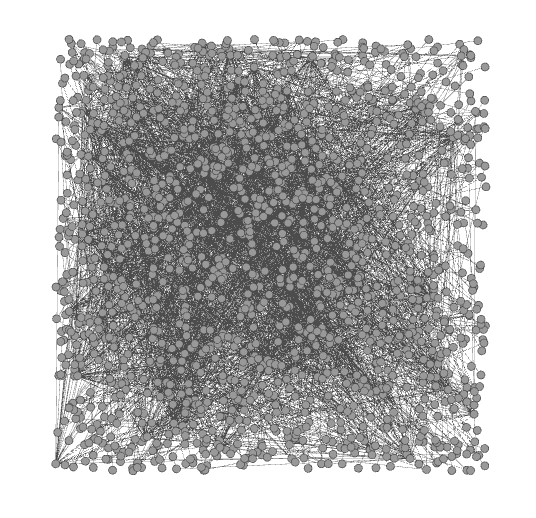
\includegraphics[width=0.47\linewidth]{./fig/doc_net_phishing.png}
\label{fig:gene_net_struct:doc_net}
}
\subfigure[Author network]{
\centering
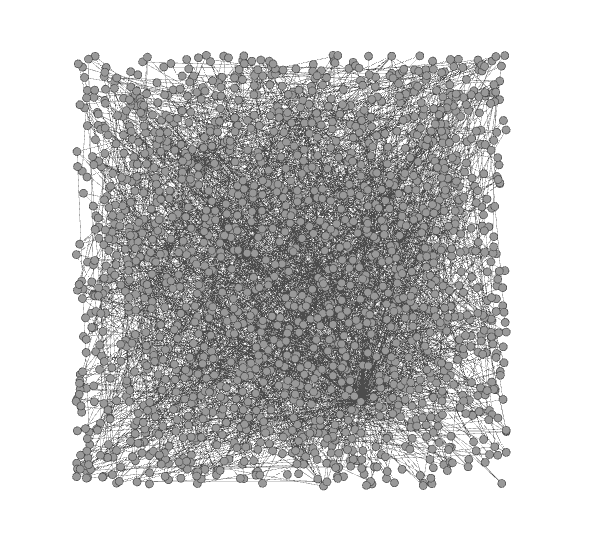
\includegraphics[width=0.47\linewidth]{./fig/auth_net_phishing.png}
\label{fig:gene_net_struct:auth_net}
} 
\caption{The network structure of the generated document network and author network.}
\label{fig:gene_net_struct}
\end{figure}

\begin{figure}[ht]
\subfigure[Document network]{
\centering
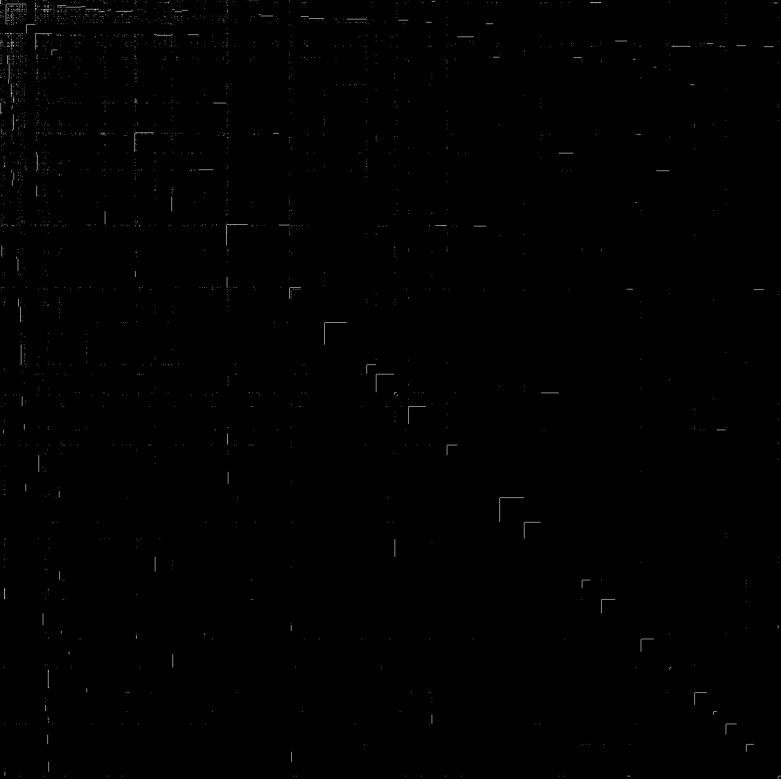
\includegraphics[width=0.47\linewidth]{./fig/doc_net_am}
\label{fig:gene_ad_mat:doc_net}
}
\subfigure[Author network]{
\centering

\includegraphics[width=0.47\linewidth]{./fig/auth_net_am}
\label{fig:gene_ad_mat:auth_net}
} 
\caption{The adjacency matrix of the generated document network and author network.}
\label{fig:gene_ad_mat}
\end{figure}

\section{Analysis}

After applying the Latent Dirichlet Allocation to the created network structure, two questions should be answered.
\begin{itemize}
\item How can the generative model be used?
\item How the generative model fits the network structure as the training data?
\end{itemize}
These two will be answered in below two subsections.

\subsection{Application}

There are several applications that we can utilize the information in the generative model.
\begin{itemize}
\item \textbf{Community discovery} \\
By looking at the probability distribution of that the actor associated with each community, an unsupervised clustering algorithm could be applied to detect potential communities among the actors. 
\item \textbf{Importance of a member in a community} \\
$ p ( \omega_{i}  \mid \iota_{j} ) $ tells the distribution of the actors given a community.
The actor with a higher probability indirectly indicates its importance in this community.
\item \textbf{Association within a community} $ p ( \iota_{j} \mid \omega_{i} ) $
It tells the probability distribution that actor $ m $ belongs to cluster $ k $.
There could be several ways to cluster the actors, e.g. using a SVM.
Here the simplest method is taken, which the community with largest probability is chosen as the one that actor belongs to.
\item \textbf{Similarity of two communities} \\
The generative model can also tell the similarity of two communities.
Because Kullback-Leibler divergence is used to measure the distance between two distributions.
The similarity between two communities can be defined as 
\begin{equation}
Sim ( \iota_{i}, \iota_{j} ) = 10^{ - \xi \ast D_{KL} ( \iota_{i}, \iota_{j} ) },
\end{equation}
in which $ D_{KL} ( \iota_{i}, \iota_{j} ) $ is
\begin{equation}
D_{KL} ( \iota_{i}, \iota_{j} ) = \sum_{k} p( \omega_{k} \mid \iota_{i} ) \log \frac{ p( \omega_{k} \mid \iota_{i} ) }{ p( \omega_{k} \mid \iota_{j} ) }.
\end{equation}
\item \textbf{Identity recognition} \\
Particularly, in the author network, the generative model can help to identify authors.
Sometimes same author shows different names in string. 
For example, some papers include the middle name, but some others does not.
The similarity of the community distribution can help to assign the papers to correct author. 

Meanwhile, different authors might have same name.
The community distribution of the papers can help to sort out the papers into different authors in different fields.
\end{itemize}

\subsection{Verification}

Before we could apply the information indicated by a generative model, we should guarantee that the generative model well approximate the training data distribution, which is the network structure in the social network analysis.
A labeled dataset with three clusters is used to verify the community discovery capability of the Latent Dirichlet Allocation.
The result is given in Figure \ref{fig:cluster3}.

In order to verify how the Latent Dirichlet Allocation applies to the social network analysis.
Two labeled dataset are also tested, which are \emph{CiteSeer} and \emph{Cora}
\footnote{The datasets are obtained from http://linqs.cs.umd.edu/projects/projects/lbc/}.
The test results are illustrated in Figure \ref{fig:doc_load01} and Figure \ref{fig:doc_load02}.
In these datasets, each paper has a label showing which community it belongs to.
After clustering the papers, we can see that the papers in the same cluster tends to share same original labels.
Because Gibbs sampling is used to train the Bayesian network of the generative model.
The convergence process could be slow.
With a longer run time, the results could shows better consistency in each cluster.

\begin{figure}[ht]
\centering
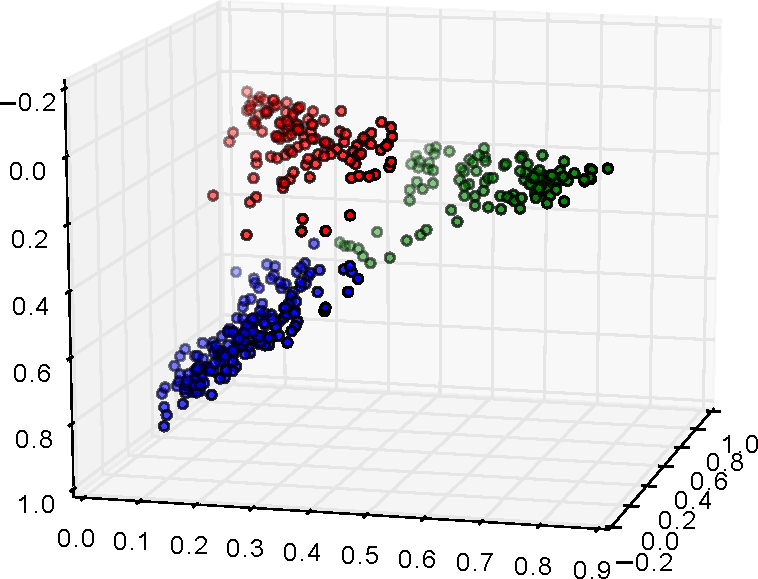
\includegraphics[width=0.8\linewidth]{./fig/cluster3}
\caption{Verify the clustering performance of Latent Dirichlet Allocation.}
\label{fig:cluster3}
\end{figure}

\begin{figure}[ht]
\subfigure[Cluster 1]{
\centering
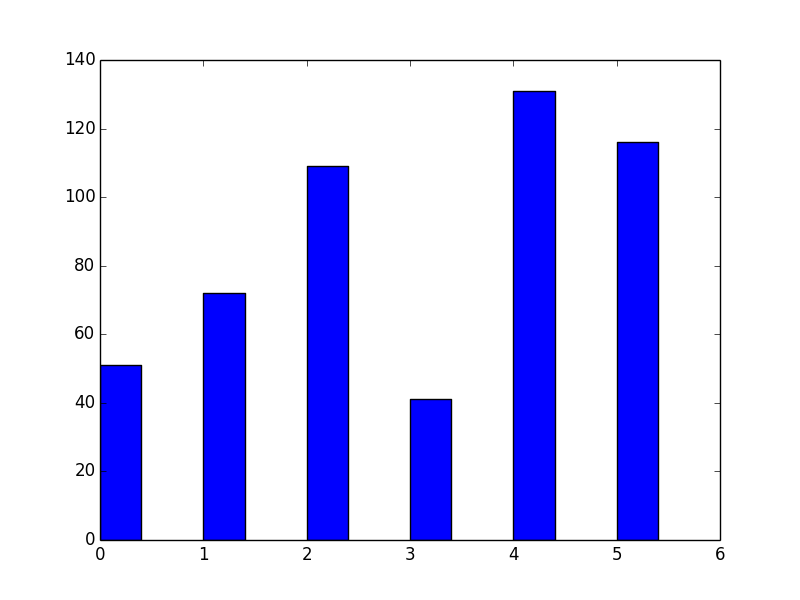
\includegraphics[width=0.3\linewidth]{./fig/doc_load01-0}
\label{fig:doc_load01:1}
}
\subfigure[Cluster 2]{
\centering
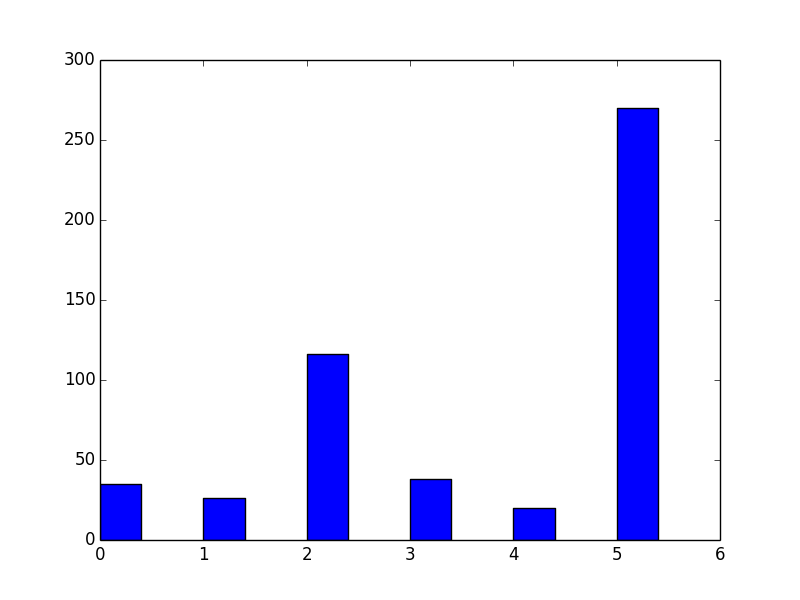
\includegraphics[width=0.3\linewidth]{./fig/doc_load01-1}
\label{fig:doc_load01:2}
} 
\subfigure[Cluster 3]{
\centering
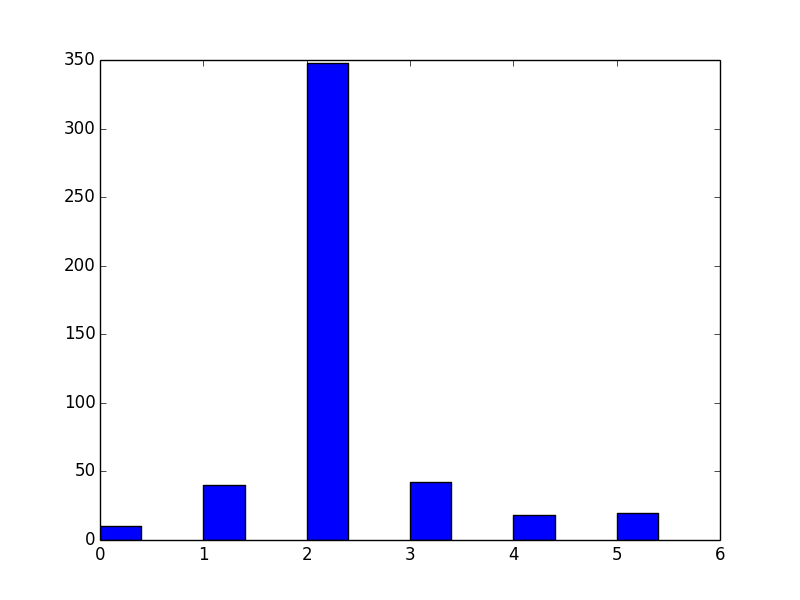
\includegraphics[width=0.3\linewidth]{./fig/doc_load01-2}
\label{fig:doc_load01:3}
}
\\
\subfigure[Cluster 4]{
\centering
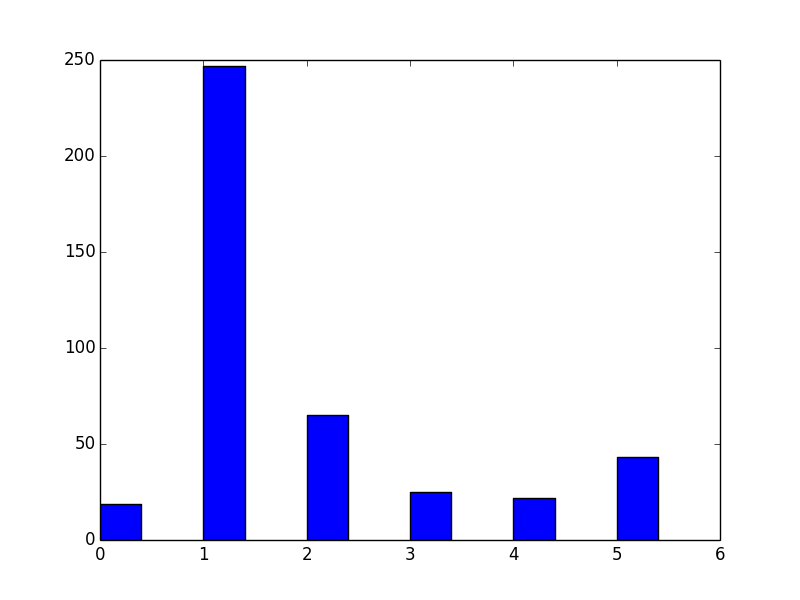
\includegraphics[width=0.3\linewidth]{./fig/doc_load01-3}
\label{fig:doc_load01:4}
}
\subfigure[Cluster 5]{
\centering
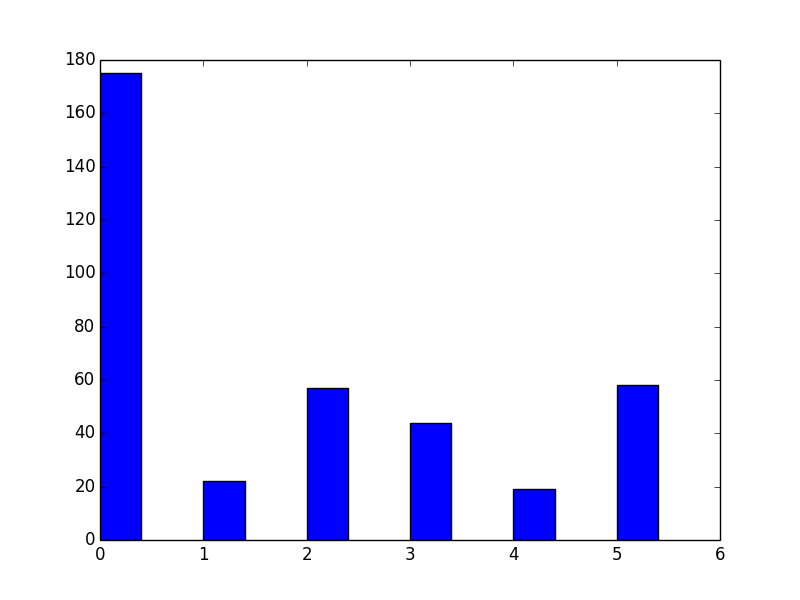
\includegraphics[width=0.3\linewidth]{./fig/doc_load01-4}
\label{fig:doc_load01:5}
} 
\subfigure[Cluster 6]{
\centering
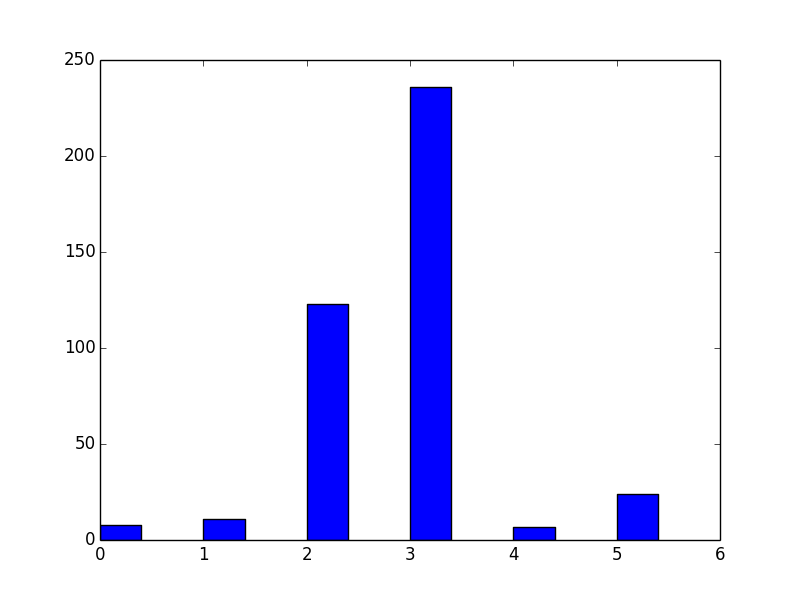
\includegraphics[width=0.3\linewidth]{./fig/doc_load01-5}
\label{fig:doc_load01:6}
}
\caption{The verification of the clusters generated from the trained generative model - \emph{cora}.}
\label{fig:doc_load01}
\end{figure}

\begin{figure}[ht]
\subfigure[Cluster 1]{
\centering
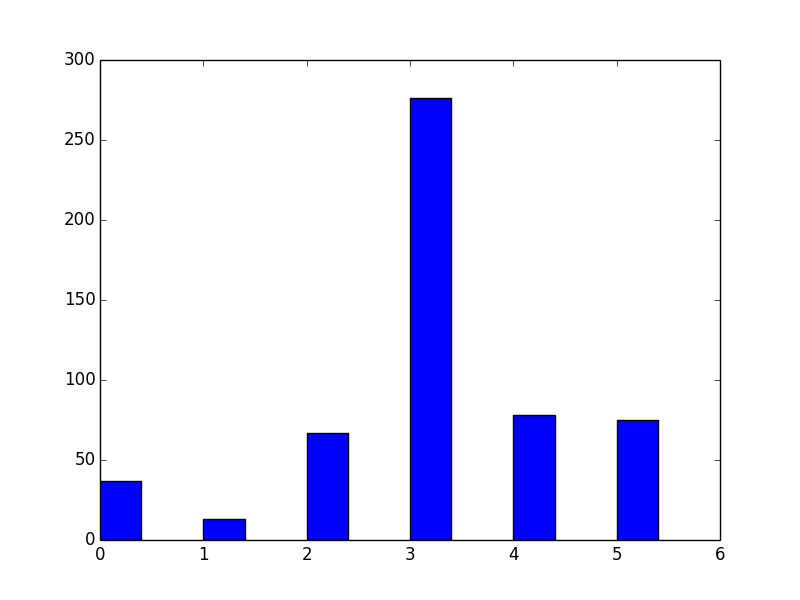
\includegraphics[width=0.3\linewidth]{./fig/doc_load02-0}
\label{fig:doc_load02:1}
}
\subfigure[Cluster 2]{
\centering
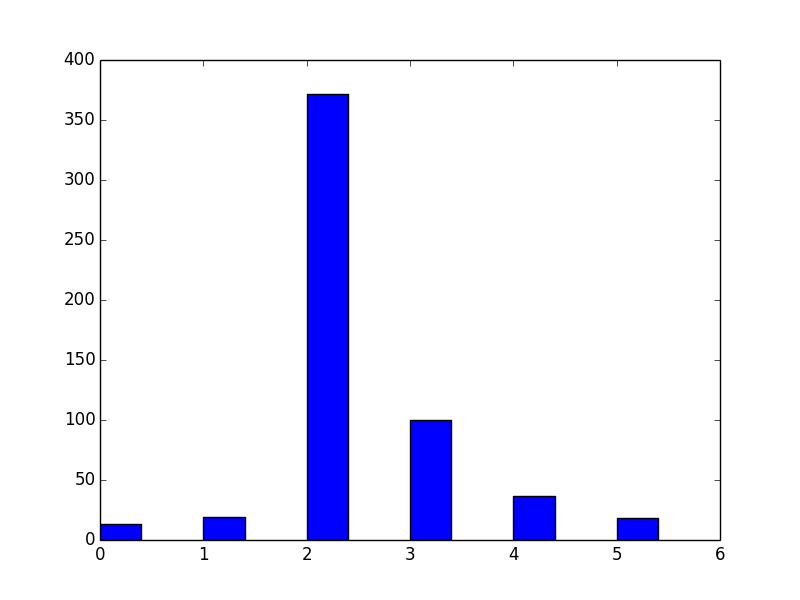
\includegraphics[width=0.3\linewidth]{./fig/doc_load02-1}
\label{fig:doc_load02:2}
} 
\subfigure[Cluster 3]{
\centering
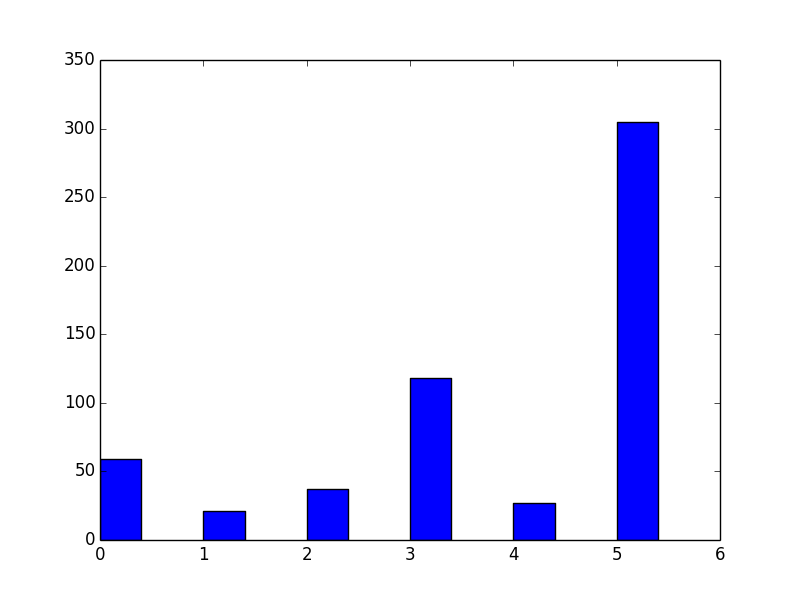
\includegraphics[width=0.3\linewidth]{./fig/doc_load02-2}
\label{fig:doc_load02:3}
}
\\
\subfigure[Cluster 4]{
\centering
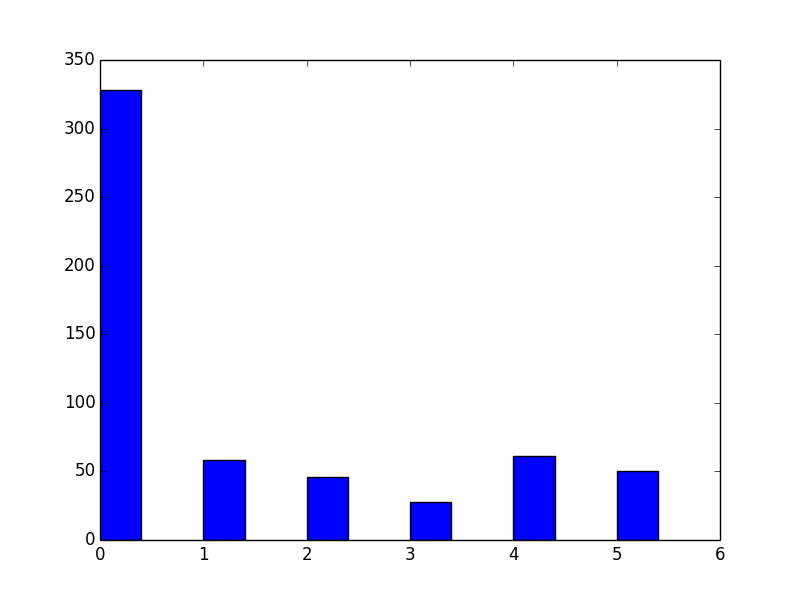
\includegraphics[width=0.3\linewidth]{./fig/doc_load02-3}
\label{fig:doc_load02:4}
}
\subfigure[Cluster 5]{
\centering
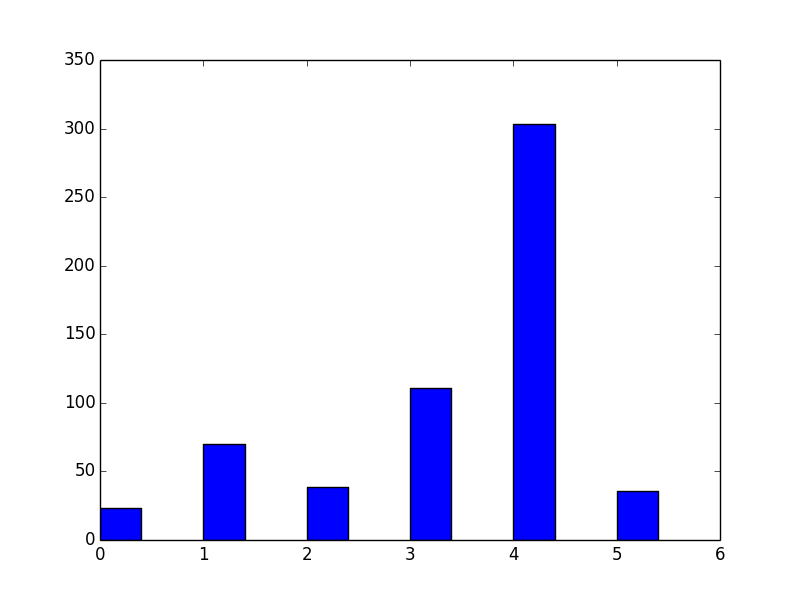
\includegraphics[width=0.3\linewidth]{./fig/doc_load02-4}
\label{fig:doc_load02:5}
} 
\subfigure[Cluster 6]{
\centering
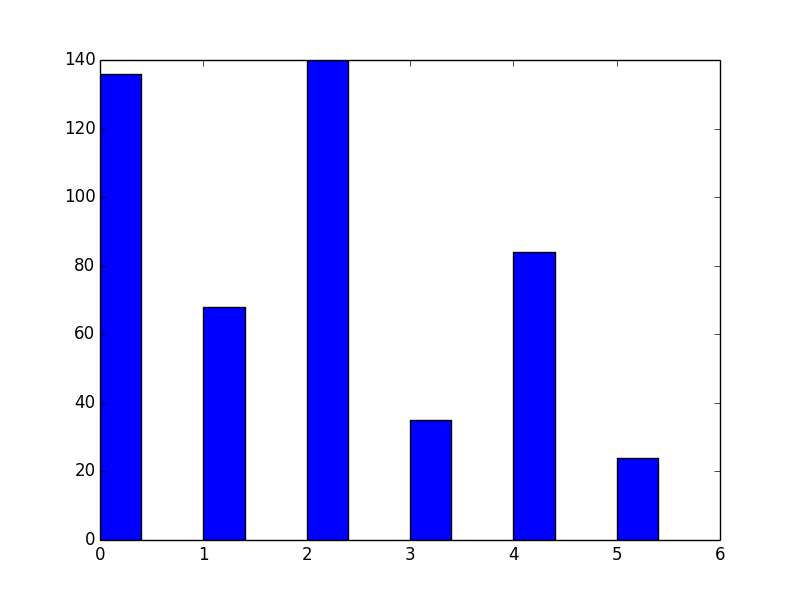
\includegraphics[width=0.3\linewidth]{./fig/doc_load02-5}
\label{fig:doc_load02:6}
}
\caption{The verification of the clusters generated from the trained generative model - \emph{CiteSeer}.}
\label{fig:doc_load02}
\end{figure}

Because there is no label assigned to the data we collected from Google Scholar.
It becomes hard to verify whether the clustering result is a good one.
Usually we need to have both a training dataset and a testing dataset.
After trained the generative model using the training dataset, the testing dataset will then be used to verify the approximative capability of the generative model.
\emph{Perplexity} is a popular metric in measuring how well the trained model fits a test dataset, which has been applied in \cite{Cha:2012:SAU:2348283.2348360} and \cite{4258697}.
It is defined as 
\begin{equation}
Perplexity( E_{test} ) = \exp^{- \frac{ \sum_{e \in E_{test}} \log p(e) }{ | E_{test} | } }
\end{equation}
Due to the time limitation, it is not tested in this project.

\section{Summary}


\bibliographystyle{abbrv}
\bibliography{reference}

\section{Appendix}
\label{sec:appendix}

Here is a list of notations.
\begin{itemize}
	\item $ M $ : number of social actors (social interaction profiles) in the social network
	\item $ K $ : number of communities (mixture components)
	\item $ N_{i} $ : number of social interactions in a social interaction profile $ \mbox{sip}_{i} $
	\item $ \vec{\alpha} $ : Dirichlet prior hyperparameter
	\item $ \vec{\beta} $ : Dirichlet prior hyperparameter
	\item $ \iota $ : hidden community variable, $ \iota_{i,j} $ means the community for the $ j $th social interaction in $ \mbox{sip}_{i} $
	\item $ \vec{\theta} $ : $ p(\iota \mid \mbox{sip}_{j}) $ is the community mixture proportion for $ \mbox{sip}_{j} $ 
	\item $ \vec{\Phi}_{k} $ : $ p(\omega \mid \iota_{k} ) $ is the mixture component of community $ k $
	\item $ \omega $ : social interaction variable, $ $ means the $ j $th social interaction in $ \mbox{sip}_{i} $
\end{itemize}

\end{document}
